\documentclass[pdftex,12pt,xcolor=svgnames]{beamer}

\mode<presentation>
{
  \usetheme{boxes}
  \usecolortheme[named=MidnightBlue]{structure}
  %\setbeamercolor{normal text}{bg=NavajoWhite!20}
  \usefonttheme{serif}
  \setbeamertemplate{navigation symbols}{}
  % Show frame number and author name in footline
  \setbeamertemplate{footline}[frame number]
  \addtobeamertemplate{footline}{\quad\textcolor{gray}{James Robert Lloyd}}{}
  % Set frame titles in small capitals
  \setbeamerfont{frametitle}{shape=\scshape,family=\rmfamily,size={\fontsize{16}{20}}}
  \setbeamercolor{frametitle}{bg=gray!60!white,fg=black}
  % Alerted text: blue (uncomment second line if theme sets alerted text to bold)
  \setbeamercolor{alerted text}{fg=blue}
  %\setbeamerfont*{alerted text}{}
  \setbeamertemplate{bibliography item}[text] %{\hbox{\donotcoloroutermaths$\blacktriangleright$}}
  \setbeamertemplate{bibliography entry title}{}
  \setbeamertemplate{bibliography entry author}{}
  \setbeamertemplate{bibliography entry note}{}
  \setbeamertemplate{bibliography entry location}{}

}
\usepackage[english]{babel}
\usepackage[latin1]{inputenc}
\usepackage{times}
\usepackage[T1]{fontenc}
\usepackage{hyperref}
\usepackage{multimedia}
\usepackage{eepic}
\usepackage{graphicx}
%\usepackage[nohug]{latexinclude/diagrams}
\usepackage{tikz}
\usetikzlibrary{calc}

%% \newcommand{\footlineextra}[1]{
%%     \begin{tikzpicture}[remember picture,overlay]
%%         \node[yshift=1.5ex,anchor=south east] at (current page.south east)
%% {#1};
%%     \end{tikzpicture}
%% }

\newcommand{\footlineextra}[1]{
    \begin{tikzpicture}[remember picture,overlay]
        \node[xshift=-5ex,yshift=-0.5ex,anchor=south east] at (current page.south east)
             {\mbox{\tiny \textcolor{MidnightBlue}{#1}}};
    \end{tikzpicture}
}

\def\sectionframe#1{
  {
    \setbeamertemplate{footline}{\empty}
    \begin{frame}{}
      \begin{center}
        \huge\sc #1
      \end{center}
    \end{frame}
  }
}


\usepackage{etex}

\usepackage{tabularx}
\usepackage{include/picins}
\usepackage{include/preamble}
\usepackage{xcolor}
\usepackage{tikz}

\usetikzlibrary{shapes.geometric,arrows,chains,matrix,positioning,scopes,calc}

%%%%%%%%%%%%%%%%%%%%%%%%%%%%%%%%%%%%%%%%%%%
%
% Some look and feel definitions
%
%%%%%%%%%%%%%%%%%%%%%%%%%%%%%%%%%%%%%%%%%%%

\setlength{\columnsep}{0.03\textwidth}
\setlength{\columnseprule}{0.0018\textwidth}
\setlength{\parindent}{0.0cm}
  
\tikzstyle{mybox} = [draw=white, rectangle]
\tikzset{hide on/.code={\only<#1>{\color{white}}}}

\definecolor{camlightblue}{rgb}{0.601 , 0.8, 1}
\definecolor{camdarkblue}{rgb}{0, 0.203, 0.402}
\definecolor{camred}{rgb}{1, 0.203, 0}
\definecolor{camyellow}{rgb}{1, 0.8, 0}
\definecolor{lightblue}{rgb}{0, 0, 0.80}
\definecolor{white}{rgb}{1, 1, 1}
\definecolor{whiteblue}{rgb}{0.80, 0.80, 1}

\newcolumntype{x}[1]{>{\centering\arraybackslash\hspace{0pt}}m{#1}}
\newcommand{\tabbox}[1]{#1}

\hypersetup{colorlinks=true,citecolor=blue}

%%%%%%%%%%%%%%%%%%%%%%%%%%%%%%%%%%%%%%%%%%%
%
% The talk
%
%%%%%%%%%%%%%%%%%%%%%%%%%%%%%%%%%%%%%%%%%%%

\title{Automatic statistical model construction, description and criticism}

\author{James Robert Lloyd}

\institute{Machine Learning Group, Department of Engineering, University of Cambridge, UK}

\begin{document}

\frame[plain] {
\titlepage
}

\begin{frame}{Credit where credit is due}

\begin{center}
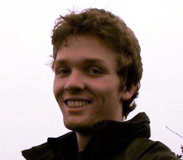
\includegraphics[height=0.2\textwidth]{figures/JamesLloyd4}
\qquad
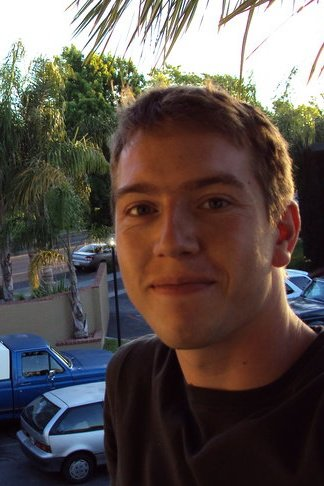
\includegraphics[height=0.2\textwidth, trim=20mm 25mm 0mm 25mm, clip]{figures/david2}
\qquad
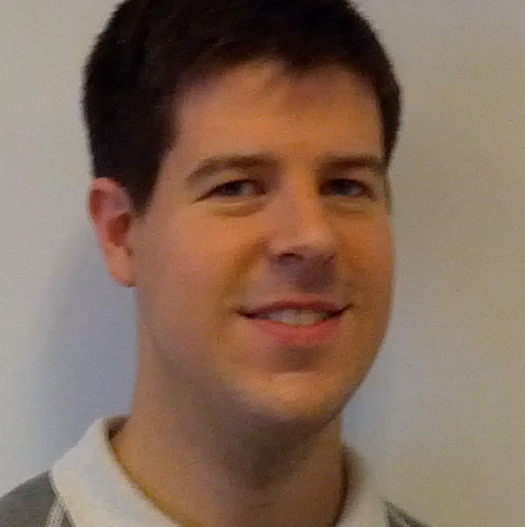
\includegraphics[height=0.2\textwidth]{figures/roger-photo}
\\
James Robert Lloyd, David Duvenaud, Roger Grosse
\end{center}
\begin{center}
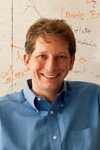
\includegraphics[height=0.2\textwidth, trim=0mm 7mm 0mm 0mm, clip]{figures/josh2}
\qquad
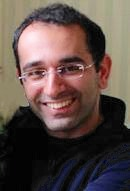
\includegraphics[height=0.2\textwidth]{figures/zg2}
\\
Joshua Tenenbaum, Zoubin Ghahramani
\end{center}

\end{frame}

\begin{frame}{What would an automatic statistician do?}
    % Define block styles
  \tikzstyle{block} = [rectangle, draw, fill=blue!20, 
                       text width=4.4em, text centered, rounded corners, minimum height=3em]
  \tikzstyle{line} = [draw, -latex']
  \tikzstyle{cloud} = [draw, ellipse,fill=red!20,minimum height=2em]
    
  \begin{tikzpicture}[node distance = 2.3cm]
    \footnotesize
    % Place nodes
    \node [cloud] (data) {Data};
    \node [block, right of=data] (search) {Search};
    \node [cloud, above of=search] (language) {Language of models};
    \node [block, below of=search] (eval) {Evaluation};
    \node [cloud, right of=search] (model) {Model};
    \node [block, right of=model] (pred) {Prediction};
    \node [block, above of=pred] (trans) {Description};
    \node [block, below of=pred] (checking) {Checking};
    \node [cloud, right of=pred] (report) {Report};
    % Draw edges
    \path [line] (data) -- (search);
    \path [line] (language) -- (search);
    \path [line] (search) -- (model);
    \path [line] (search) -- (model);
    \path [line] (model.north east) -- (trans.south west);
    \path [line] (model.east) -- (pred.west);
    \path [line] (model.south east) -- (checking.north west);
    \path [line] (trans.south east) -- (report.north west);
    \path [line] (pred.east) -- (report.west);
    \path [line] (checking.north east) -- (report.south west);
    \draw[->,] (search.south east) .. controls (3.45,-1.15) .. (eval.north east);
    \draw[->,] (eval.north west) .. controls (1.15,-1.15) .. (search.south west);
  \end{tikzpicture}
\end{frame}

\begin{frame}{Preview: An entirely automatic analysis}

\newcommand{\wmgd}{0.5\columnwidth}
\newcommand{\hmgd}{3.0cm}
\newcommand{\mdrd}{figures/01-airline}
\newcommand{\mbm}{\hspace{-0.3cm}}
\begin{tabular}{cc}
\mbm 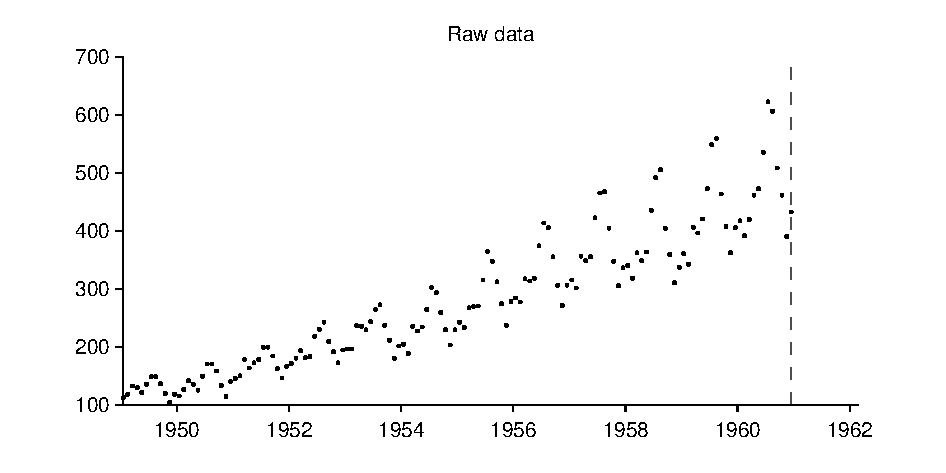
\includegraphics[width=\wmgd,height=\hmgd]{\mdrd/01-airline_raw_data} & \includegraphics[width=\wmgd,height=\hmgd]{\mdrd/01-airline_all}
\end{tabular}
\vspace{0.5\baselineskip}

{\footnotesize
Four additive components have been identified in the data
\begin{itemize}
  \item A linearly increasing function. 
  \item An approximately periodic function with a period of 1.0 years and with linearly increasing amplitude. 
  \item A smooth function. 
  \item Uncorrelated noise with linearly increasing standard deviation. 
\end{itemize}
}
\end{frame}

\begin{frame}{Agenda}
  \begin{itemize}
    \item Automatic model building via a grammar on kernels
    \vspace{\baselineskip}
    \item Automatically describing models in natural language
    \vspace{\baselineskip}
    \item A mostly automatic model criticism procedure
    \vspace{\baselineskip}
    \item Future directions and challenges
  \end{itemize}
\end{frame}

\begin{frame}{Gaussian processes: the usual story}
  We assume that our data is generated from a zero mean Gaussian process with squared exponential kernel plus independent Gaussian noise
  \vspace{\baselineskip}
  \begin{center}
    \includegraphics<1>[width=0.8\textwidth]{figures/lin_reg/sq_exp_prior}
    \includegraphics<2>[width=0.8\textwidth]{figures/quad/sq_exp_1}
    \includegraphics<3>[width=0.8\textwidth]{figures/quad/sq_exp_2}
    \includegraphics<4>[width=0.8\textwidth]{figures/quad/sq_exp_3}
    \includegraphics<5>[width=0.8\textwidth]{figures/quad/sq_exp_5}
    \includegraphics<6>[width=0.8\textwidth]{figures/quad/sq_exp_10}
    \includegraphics<7>[width=0.8\textwidth]{figures/quad/sq_exp_15}
  \end{center}
\end{frame}

\begin{frame}{More complex kernels required}
  \begin{center}
    \only<1>{Long lengthscale SE}
    \only<2>{Short lengthscale SE}
    \only<3>{Long lengthscale SE + Short lengthscale SE}
    \only<4>{SE + SE + SE + SE $\times$ Periodic}
  \end{center}
  \begin{center}
    \includegraphics<1>[width=0.8\textwidth]{figures/mauna-plots/SE-long.pdf}
    \includegraphics<2>[width=0.8\textwidth]{figures/mauna-plots/SE-short.pdf}
    \includegraphics<3>[width=0.8\textwidth]{figures/mauna-plots/SE-SE.pdf}
    \includegraphics<4>[width=0.8\textwidth]{figures/mauna-plots/Complex.pdf}
  \end{center}
\end{frame}

\begin{frame}{Defining a language of models}
    % Define block styles
  \tikzstyle{block} = [rectangle, draw, fill=blue!20, 
                       text width=4.4em, text centered, rounded corners, minimum height=3em]
  \tikzstyle{line} = [draw, -latex']
  \tikzstyle{cloud} = [draw, ellipse,fill=red!20,minimum height=2em]
  \tikzstyle{supercloud} = [draw, ellipse,fill=red!50,minimum height=2em,]
    
  \begin{tikzpicture}[node distance = 2.3cm]
    \footnotesize
    % Place nodes
    \node [cloud] (data) {Data};
    \node [block, right of=data] (search) {Search};
    \node [supercloud, above of=search] (language) {\bf Language of models};
    \node [block, below of=search] (eval) {Evaluation};
    \node [cloud, right of=search] (model) {Model};
    \node [block, right of=model] (pred) {Prediction};
    \node [block, above of=pred] (trans) {Description};
    \node [block, below of=pred] (checking) {Checking};
    \node [cloud, right of=pred] (report) {Report};
    % Draw edges
    \path [line] (data) -- (search);
    \path [line] (language) -- (search);
    \path [line] (search) -- (model);
    \path [line] (search) -- (model);
    \path [line] (model.north east) -- (trans.south west);
    \path [line] (model.east) -- (pred.west);
    \path [line] (model.south east) -- (checking.north west);
    \path [line] (trans.south east) -- (report.north west);
    \path [line] (pred.east) -- (report.west);
    \path [line] (checking.north east) -- (report.south west);
    \draw[->,] (search.south east) .. controls (3.45,-1.15) .. (eval.north east);
    \draw[->,] (eval.north west) .. controls (1.15,-1.15) .. (search.south west);
  \end{tikzpicture}
\end{frame}

\begin{frame}{The atoms of our language}  
  \newcommand{\fhbig}{1.0cm}
\newcommand{\fwbig}{1.2cm}
\newcommand{\kernpic}[1]{\includegraphics[height=\fhbig,width=\fwbig]{figures/structure_examples/#1}}
\newcommand{\colsize}{1.7cm}
\newcommand{\sepsize}{0.0cm}

Five base kernels

\vspace{\baselineskip}

\begin{tabularx}{\columnwidth}{x{\colsize}x{\colsize}x{\colsize}x{\colsize}x{\colsize}}
  \kernpic{se_kernel} & \kernpic{per_kernel} & \kernpic{lin_kernel} & \kernpic{c_kernel} & \kernpic{wn_kernel} \\
  {\footnotesize Squared \newline exp. (\kSE)} & {\footnotesize Periodic (\kPer)} & {\footnotesize Linear (\kLin)} & {\footnotesize Constant (\kC)} & {\footnotesize White \newline noise (\kWN)}
\end{tabularx}

\vspace{\baselineskip}

Encoding for the following types of functions

\vspace{\baselineskip}

\begin{tabularx}{\columnwidth}{x{\colsize}x{\colsize}x{\colsize}x{\colsize}x{\colsize}}
  \kernpic{se_kernel_draws} & \kernpic{per_kernel_draws_s2} & \kernpic{lin_kernel_draws} & \kernpic{c_kernel_draws} & \kernpic{wn_kernel_draws} \\
  {\footnotesize Smooth \newline functions} & {\footnotesize Periodic functions} & {\footnotesize Linear \newline functions} & {\footnotesize Constant \newline functions} & {\footnotesize Gaussian \newline noise} 
\end{tabularx}


\end{frame}

\begin{frame}{The composition rules of our language}
\begin{itemize} 
	\item Two main operations: addition, multiplication
\end{itemize}
\newcommand{\fhbig}{1.6cm}
\newcommand{\fwbig}{1.8cm}
\newcommand{\kernpic}[1]{\includegraphics[height=\fhbig,width=\fwbig]{figures/structure_examples/#1}}
\newcommand{\largeplus}{\tabbox{{\Large+}}}
\newcommand{\largeeq}{\tabbox{{\Large=}}}
\newcommand{\largetimes}{\tabbox{{\Large$\times$}}}
\begin{figure}[ht]
\centering
\renewcommand{\tabularxcolumn}[1]{>{\arraybackslash}m{#1}}
\begin{tabularx}{\columnwidth}{XXcXX}
  \kernpic{lin_times_lin} & \kernpic{lin_times_lin_draws} & \phantom{mm}
& \kernpic{longse_times_per} & \kernpic{longse_times_per_draws_s1}
\\
  {\small $\kLin \times \kLin$} & {\small quadratic functions} & \phantom{mm}
& {\small $\kSE \times \kPer$} & {\small locally \newline periodic}
\\ \\
%\midrule 
  \kernpic{lin_plus_per} & \kernpic{lin_plus_per_draws} & \phantom{mm} 
& \kernpic{se_plus_per} & \kernpic{se_plus_per_draws_s7}
\\
  {\small $\kLin + \kPer$} & {\small periodic plus linear trend} & \phantom{mm}
& {\small $\kSE + \kPer$ } & {\small periodic plus smooth trend}
\end{tabularx}
\end{figure}


\end{frame}

\begin{frame}{Modeling changepoints}
  
  Time series data often exhibit changepoints:
  
  \begin{center}
  \begin{tabular}{cc}
    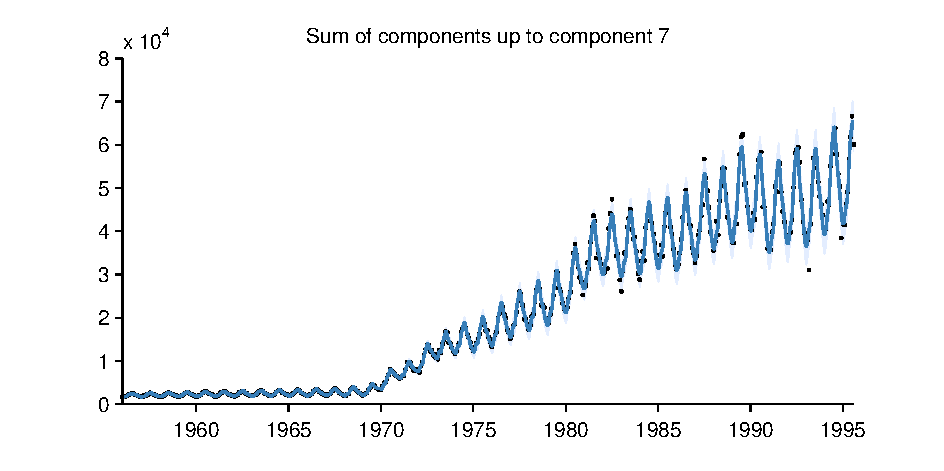
\includegraphics[width=0.4\textwidth]{figures/09-gas-production_7_cum} &
    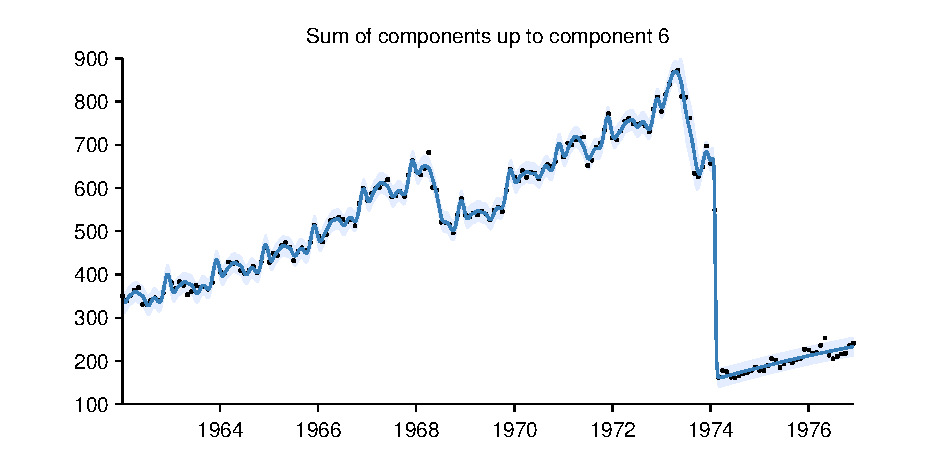
\includegraphics[width=0.4\textwidth]{figures/07-call-centre_6_cum} 
  \end{tabular}
  \end{center}
  
  \pause

  We can model this by assuming $\textcolor{red}{f_1(x)} \sim \gp{}(0,k_1)$ and $\textcolor{blue}{f_2(x)} \sim \gp{}(0,k_2)$ and then defining
\[
f(x) = (1-\sigma(x))\, \textcolor{red}{f_1(x)} + \sigma(x)\, \textcolor{blue}{f_2(x)}
\]

where $\sigma$ is a sigmoid function between 0 and 1.
\end{frame}

\begin{frame}{Modeling changepoints}
  We can model this by assuming $\textcolor{red}{f_1(x)} \sim \gp{}(0,k_1)$ and $\textcolor{blue}{f_2(x)} \sim \gp{}(0,k_2)$ and then defining
\[
f(x) = (1-\sigma(x))\, \textcolor{red}{f_1(x)} + \sigma(x)\, \textcolor{blue}{f_2(x)}
\]

where $\sigma$ is a sigmoid function between 0 and 1.

\vspace{2\baselineskip}

Then $f \sim \gp{}(0,k)$, where
\[
k(x,x') = (1-\sigma(x)) \, \textcolor{red}{k_1(x,x')}  \, (1-\sigma(x')) + \sigma(x) \,
\textcolor{blue}{k_2(x,x')} \, \sigma(x') 
\]

We define the changepoint operator $\kernel = \kCP(\kernel_1, \kernel_2)$.

\end{frame}

\begin{frame}{An expressive language of models}
\begin{center}
\begin{tabular}{l|l}
Regression model & Kernel \\
\midrule
\gp{} smoothing & $\kSE + \kWN$ \\
Linear regression & $\kC + \kLin + \kWN$ \\
Multiple kernel learning & $\sum \kSE$ + \kWN\\
Trend, cyclical, irregular & $\sum \kSE + \sum \kPer$ + \kWN\\
Fourier decomposition & $\kC + \sum \cos$ + \kWN\\
Sparse spectrum \gp{}s & $\sum \cos$ + \kWN\\
Spectral mixture & $\sum \SE \times \cos$ + \kWN\\
Changepoints & \eg $\kCP(\kSE, \kSE) + \kWN$ \\
Heteroscedasticity & \eg $\kSE + \kLin \times \kWN$
\end{tabular}
\end{center}
Note: $\cos$ is a special case of our version of $\kPer$
\end{frame}

\begin{frame}{Discovering a good model via search}
    % Define block styles
  \tikzstyle{block} = [rectangle, draw, fill=blue!20, 
                       text width=4.4em, text centered, rounded corners, minimum height=3em]
  \tikzstyle{superblock} = [rectangle, draw, fill=blue!50, 
                       text width=4.4em, text centered, rounded corners, minimum height=3em]
  \tikzstyle{line} = [draw, -latex']
  \tikzstyle{cloud} = [draw, ellipse,fill=red!20,minimum height=2em]
  \tikzstyle{supercloud} = [draw, ellipse,fill=red!50,minimum height=2em]
    
  \begin{tikzpicture}[node distance = 2.3cm]
    \footnotesize
    % Place nodes
    \node [cloud] (data) {Data};
    \node [superblock, right of=data] (search) {\bf Search};
    \node [cloud, above of=search] (language) {Language of models};
    \node [block, below of=search] (eval) {Evaluation};
    \node [cloud, right of=search] (model) {Model};
    \node [block, right of=model] (pred) {Prediction};
    \node [block, above of=pred] (trans) {Description};
    \node [block, below of=pred] (checking) {Checking};
    \node [cloud, right of=pred] (report) {Report};
    % Draw edges
    \path [line] (data) -- (search);
    \path [line] (language) -- (search);
    \path [line] (search) -- (model);
    \path [line] (search) -- (model);
    \path [line] (model.north east) -- (trans.south west);
    \path [line] (model.east) -- (pred.west);
    \path [line] (model.south east) -- (checking.north west);
    \path [line] (trans.south east) -- (report.north west);
    \path [line] (pred.east) -- (report.west);
    \path [line] (checking.north east) -- (report.south west);
    \draw[->,] (search.south east) .. controls (3.45,-1.15) .. (eval.north east);
    \draw[->,] (eval.north west) .. controls (1.15,-1.15) .. (search.south west);
  \end{tikzpicture}
\end{frame}

\begin{frame}{Discovering a good model via search}
  \begin{itemize}
    \item Language defined as the arbitrary composition of five base kernels ($\kWN, \kC, \kLin, \kSE, \kPer$) via three operators ($+, \times, \kCP$). 
    \vspace{\baselineskip}
    \item The space spanned by this language is open-ended and can have a high branching factor requiring a judicious search
    \vspace{\baselineskip}
    \item We propose a greedy search for its simplicity and similarity to human model-building
  \end{itemize}
\end{frame}

\begin{frame}{Example: Mauna Loa Keeling Curve}
\hspace{-1.2cm}
\only<1>{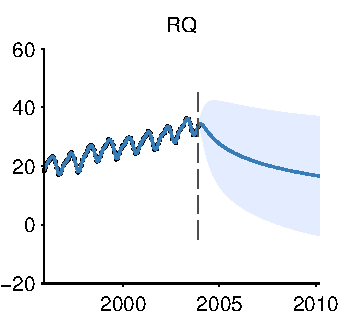
\includegraphics[width=0.4\textwidth]{figures/11-Feb-v4-03-mauna2003-s_max_level_0/03-mauna2003-s_all_small.pdf}}
\only<2>{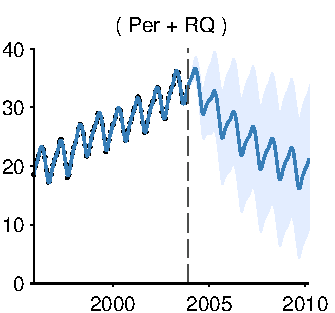
\includegraphics[width=0.4\textwidth]{figures/11-Feb-v4-03-mauna2003-s_max_level_1/03-mauna2003-s_all_small.pdf}}
\only<3>{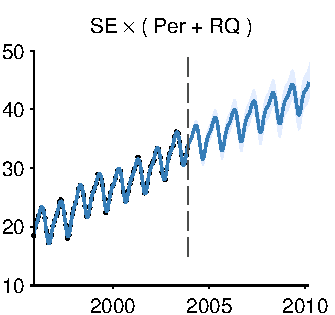
\includegraphics[width=0.4\textwidth]{figures/11-Feb-v4-03-mauna2003-s_max_level_2/03-mauna2003-s_all_small.pdf}}
\only<4>{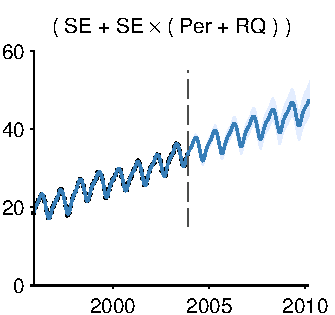
\includegraphics[width=0.4\textwidth]{figures/11-Feb-v4-03-mauna2003-s_max_level_3/03-mauna2003-s_all_small.pdf}}

\vspace{-3.5cm}
\begin{minipage}[t][14cm][t]{1.14\linewidth}
\begin{flushleft}
\hspace{5.5cm}
\vspace{-8cm}
\makebox[\textwidth][c]{
\raisebox{10cm}{
\vspace{-8cm}
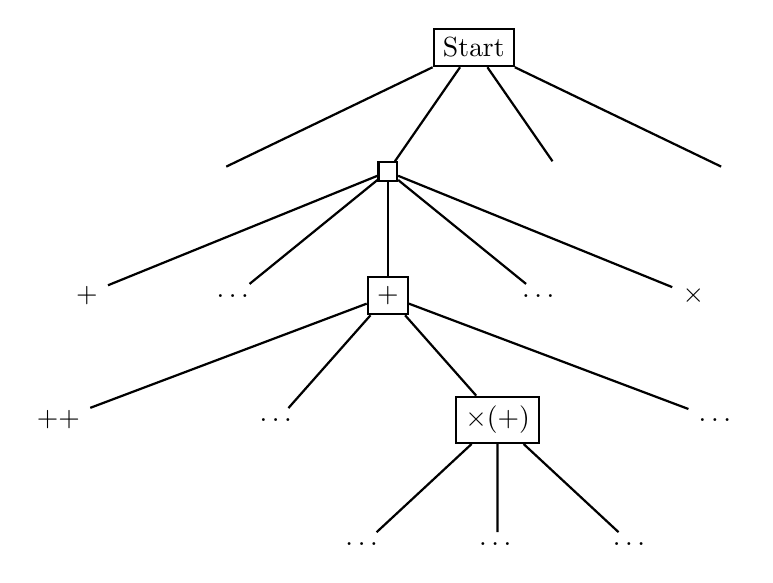
\begin{tikzpicture}
[sibling distance=0.18\columnwidth,-,thick, level distance=0.13\columnwidth]
%\footnotesize
\node[shape=rectangle,draw,thick] {Start}
%\pause
  child {node {$\SE$}}
%  fill=camlightblue!30
  child {node[shape=rectangle,draw,thick] {$\RQ$}
    [sibling distance=0.16\columnwidth]
%    {\visible<2->{ child {node {\ldots}}}}
    child [hide on=-1] {node {$\SE$ + \RQ}}
    child [hide on=-1] {node {\ldots}}
    child [hide on=-1] {node[shape=rectangle,draw,thick] {$\Per + \RQ$}
      [sibling distance=0.23\columnwidth]
      child [hide on=-2] {node {$\SE + \Per + \RQ$}}
      child [hide on=-2] {node {\ldots}}
      child [hide on=-2] {node[shape=rectangle,draw,thick] {$\SE \times (\Per + \RQ)$}
        [sibling distance=0.14\columnwidth]
        child [hide on=-3] {node {\ldots}}
        child [hide on=-3] {node {\ldots}}
        child [hide on=-3] {node {\ldots}}
      }
      child [hide on=-2] {node {\ldots}}
    }
    %child {node {$\RQ \times \SE$}}
    child [hide on=-1] {node {\ldots}}
    child [hide on=-1] {node {$\Per \times \RQ$}}
  }
  child {node {$\Lin$}}
  child {node {$\Per$}}
  ;
\end{tikzpicture}}
}\end{flushleft}
\end{minipage}
\only<4>{}
\end{frame}

\begin{frame}{Model evaluation}
    % Define block styles
  \tikzstyle{block} = [rectangle, draw, fill=blue!20, 
                       text width=4.4em, text centered, rounded corners, minimum height=3em]
  \tikzstyle{superblock} = [rectangle, draw, fill=blue!50, 
                       text width=4.4em, text centered, rounded corners, minimum height=3em]
  \tikzstyle{line} = [draw, -latex']
  \tikzstyle{cloud} = [draw, ellipse,fill=red!20,minimum height=2em]
  \tikzstyle{supercloud} = [draw, ellipse,fill=red!50,minimum height=2em]
    
  \begin{tikzpicture}[node distance = 2.3cm]
    \footnotesize
    % Place nodes
    \node [cloud] (data) {Data};
    \node [block, right of=data] (search) {Search};
    \node [cloud, above of=search] (language) {Language of models};
    \node [superblock, below of=search] (eval) {\bf Evaluation};
    \node [cloud, right of=search] (model) {Model};
    \node [block, right of=model] (pred) {Prediction};
    \node [block, above of=pred] (trans) {Description};
    \node [block, below of=pred] (checking) {Checking};
    \node [cloud, right of=pred] (report) {Report};
    % Draw edges
    \path [line] (data) -- (search);
    \path [line] (language) -- (search);
    \path [line] (search) -- (model);
    \path [line] (search) -- (model);
    \path [line] (model.north east) -- (trans.south west);
    \path [line] (model.east) -- (pred.west);
    \path [line] (model.south east) -- (checking.north west);
    \path [line] (trans.south east) -- (report.north west);
    \path [line] (pred.east) -- (report.west);
    \path [line] (checking.north east) -- (report.south west);
    \draw[->,] (search.south east) .. controls (3.45,-1.15) .. (eval.north east);
    \draw[->,] (eval.north west) .. controls (1.15,-1.15) .. (search.south west);
  \end{tikzpicture}
\end{frame}

\begin{frame}{Model evaluation}
  \begin{itemize}
    \item After proposing a new model its kernel parameters are optimised by conjugate gradients
    \vspace{\baselineskip}
    \item We evaluate each optimised model, $M$, using the \textcolor{red}{marginal likelihood} which can be computed analytically for \gp{}s
    \vspace{\baselineskip}
    \item We \textcolor{blue}{penalise} the marginal likelihood for the \textcolor{blue}{optimised kernel parameters} using the Bayesian Information Criterion (BIC):
\[
-0.5 \times \textrm{BIC}(M) = \textcolor{red}{\log p(D\,|\, M)} - \textcolor{blue}{\frac{p}{2} \log n}
\]
where $p$ is the number of kernel parameters, $D$ represents the data, and $n$ is the number of data points.
  \end{itemize}
\end{frame}

\begin{frame}{Automatic translation of models}
    % Define block styles
  \tikzstyle{block} = [rectangle, draw, fill=blue!20, 
                       text width=4.4em, text centered, rounded corners, minimum height=3em]
  \tikzstyle{superblock} = [rectangle, draw, fill=blue!50, 
                       text width=4.4em, text centered, rounded corners, minimum height=3em]
  \tikzstyle{line} = [draw, -latex']
  \tikzstyle{cloud} = [draw, ellipse,fill=red!20,minimum height=2em]
  \tikzstyle{supercloud} = [draw, ellipse,fill=red!50,minimum height=2em]
    
  \begin{tikzpicture}[node distance = 2.3cm]
    \footnotesize
    % Place nodes
    \node [cloud] (data) {Data};
    \node [block, right of=data] (search) {Search};
    \node [cloud, above of=search] (language) {Language of models};
    \node [block, below of=search] (eval) {Evaluation};
    \node [cloud, right of=search] (model) {Model};
    \node [block, right of=model] (pred) {Prediction};
    \node [superblock, above of=pred] (trans) {Description};
    \node [block, below of=pred] (checking) {Checking};
    \node [cloud, right of=pred] (report) {Report};
    % Draw edges
    \path [line] (data) -- (search);
    \path [line] (language) -- (search);
    \path [line] (search) -- (model);
    \path [line] (search) -- (model);
    \path [line] (model.north east) -- (trans.south west);
    \path [line] (model.east) -- (pred.west);
    \path [line] (model.south east) -- (checking.north west);
    \path [line] (trans.south east) -- (report.north west);
    \path [line] (pred.east) -- (report.west);
    \path [line] (checking.north east) -- (report.south west);
    \draw[->,] (search.south east) .. controls (3.45,-1.15) .. (eval.north east);
    \draw[->,] (eval.north west) .. controls (1.15,-1.15) .. (search.south west);
  \end{tikzpicture}
\end{frame}

\begin{frame}{Automatic translation of models}
  \begin{itemize}
    \item Search can produce {\bf arbitrarily complicated models} from open-ended language but two main properties allow description to be automated
    \vspace{\baselineskip}
    \item Kernels can be {\bf decomposed} into a {\bf sum of products}
    \begin{itemize}
      \item A sum of kernels corresponds to a sum of functions
      \item Therefore, we can describe each product of kernels separately
    \end{itemize}
    \vspace{\baselineskip}
    \item Each kernel in a product modifies a model in a {\bf consistent} way
    \begin{itemize}
      \item Each kernel roughly corresponds to an adjective
    \end{itemize}
  \end{itemize}
\end{frame}

\begin{frame}{Sum of products normal form}
  %\begin{center}
  Suppose the search finds the following kernel
  \begin{align*}
    \kSE \times (\kWN \times \kLin + \kCP(\kC, \kPer))
  \end{align*}
  \pause
  The changepoint can be converted into a sum of products
  \begin{align*}
    \kSE \times (\kWN \times \kLin + \kC \times \boldsymbol{\sigma} + \kPer \times \boldsymbol{\bar\sigma})
  \end{align*}
  \pause
  Multiplication can be distributed over addition
  \begin{align*}
    \kSE \times \kWN \times \kLin + \kSE \times \kC \times \boldsymbol{\sigma} + \kSE \times \kPer \times \boldsymbol{\bar\sigma}
  \end{align*}
  \pause
  Simplification rules are applied
  \begin{align*}
    \kWN \times \kLin + \kSE \times \boldsymbol{\sigma} + \kSE \times \kPer \times \boldsymbol{\bar\sigma}
  \end{align*}
  %\end{center}
\end{frame}

\begin{frame}{Sums of kernels are sums of functions}
  If ${\textcolor{red}{f_1} \,\sim\, \gp{}(0, \textcolor{red}{\kernel_1})}$ and independently ${\textcolor{blue}{f_2} \,\sim\, \gp{}(0, \textcolor{blue}{\kernel_2})}$ then
  \begin{align*}
  \textcolor{red}{f_1} + \textcolor{blue}{f_2} \,\sim\, \gp{}(0, \textcolor{red}{\kernel_1} + \textcolor{blue}{\kernel_2})
  \end{align*}
  
\eg

\vspace{\baselineskip}

\begin{tabular}{ccccccc}
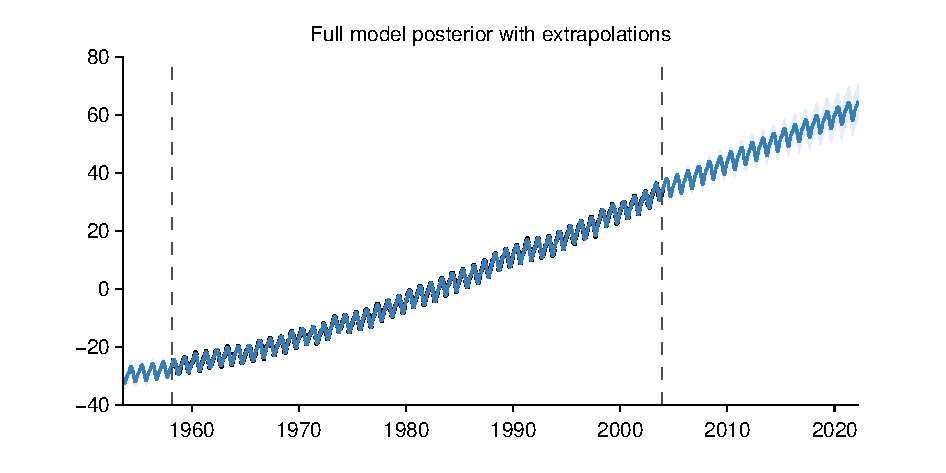
\includegraphics[trim=30 0 62 25, clip, width=0.15\textwidth]{figures/03-mauna2003_all} &
\raisebox{0.4cm}{$=$} &
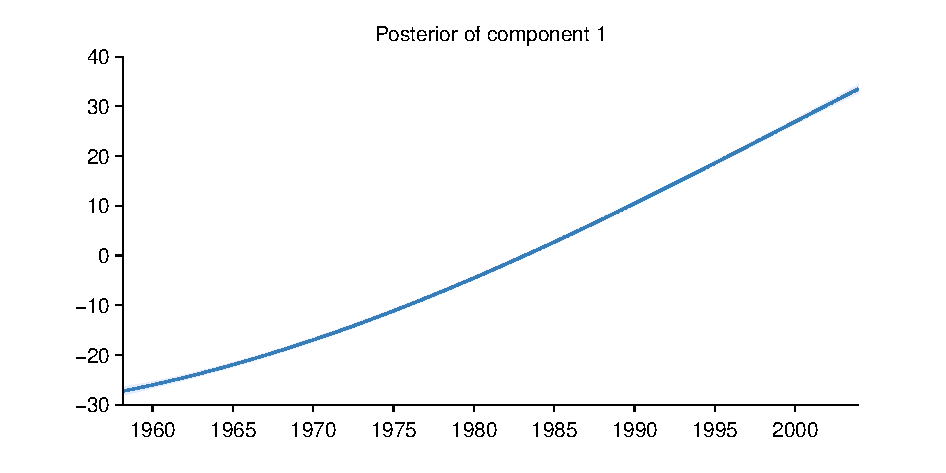
\includegraphics[trim=30 0 62 25, clip, width=0.15\textwidth]{figures/03-mauna2003_1} &
\raisebox{0.4cm}{$+$} &
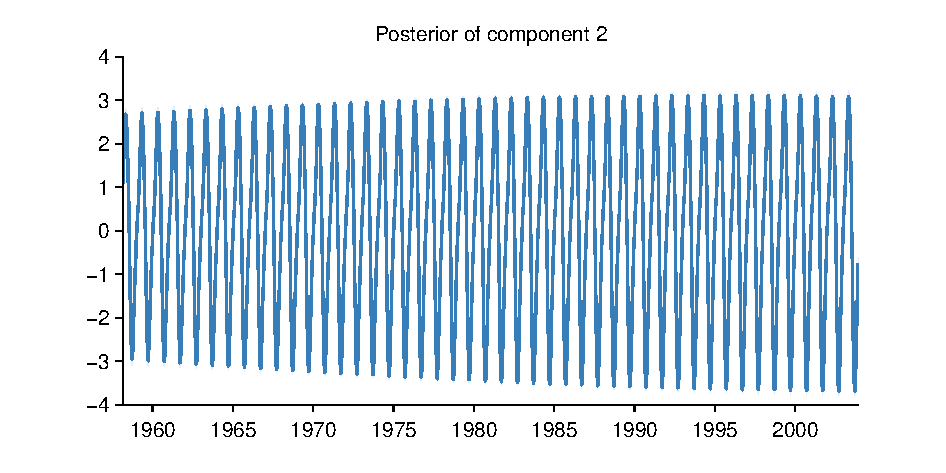
\includegraphics[trim=30 0 62 25, clip, width=0.15\textwidth]{figures/03-mauna2003_2} &
\raisebox{0.4cm}{$+$} &
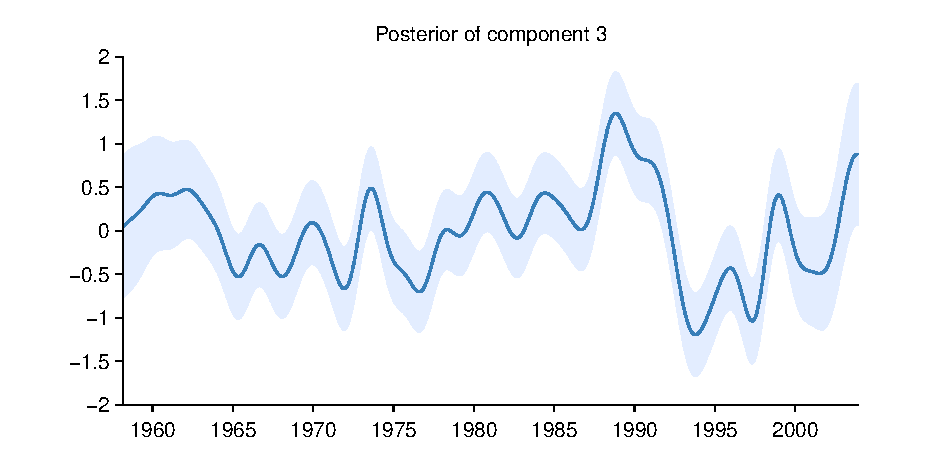
\includegraphics[trim=30 0 62 25, clip, width=0.15\textwidth]{figures/03-mauna2003_3}
\end{tabular}

\vspace{\baselineskip}

\begin{tabular}{ccccccc}
\includegraphics[trim=30 0 62 25, clip, width=0.15\textwidth]{figures/01-airline_all} &
\raisebox{0.4cm}{$=$} &
\includegraphics[trim=30 0 62 25, clip, width=0.15\textwidth]{figures/01-airline_1} &
\raisebox{0.4cm}{$+$} &
\includegraphics[trim=30 0 62 25, clip, width=0.15\textwidth]{figures/01-airline_2} &
\raisebox{0.4cm}{$+$} &
\includegraphics[trim=30 0 62 25, clip, width=0.15\textwidth]{figures/01-airline_3}
\end{tabular}

\vspace{\baselineskip}

We can therefore describe each component separately

\end{frame}

\begin{frame}{Products of kernels}
  \begin{align*}
    \phantom{\underbrace{\kSE}_{\textnormal{\scriptsize approximately}} \times }
    \underbrace{\kPer}_{\textnormal{\scriptsize periodic function}} \phantom{\times 
    \underbrace{\kLin}_{\textnormal{\scriptsize with linearly growing amplitude}} \times 
    \underbrace{\boldsymbol{\sigma}}_{\textnormal{\scriptsize until 1700}}}
  \end{align*}
  
  \vspace{\baselineskip}
  
  On their own, each kernel is described by a standard noun phrase
  
  \vspace{\baselineskip}
  
  \begin{block}{}
    \begin{tabular}{cccc}
      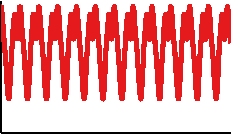
\includegraphics[width=0.2\textwidth]{figures/trans_samples/draw_11} &
      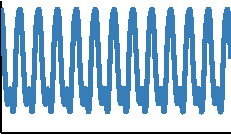
\includegraphics[width=0.2\textwidth]{figures/trans_samples/draw_12} &
      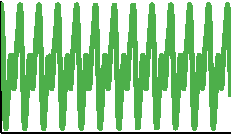
\includegraphics[width=0.2\textwidth]{figures/trans_samples/draw_13} &
      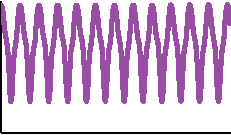
\includegraphics[width=0.2\textwidth]{figures/trans_samples/draw_14}
    \end{tabular}
  \end{block}
\end{frame}

\begin{frame}{Products of kernels - $\kSE$}
  \begin{align*}
    \underbrace{\kSE}_{\textnormal{\scriptsize approximately}} \times
    \underbrace{\kPer}_{\textnormal{\scriptsize periodic function}} \phantom{\times 
    \underbrace{\kLin}_{\textnormal{\scriptsize with linearly growing amplitude}} \times 
    \underbrace{\boldsymbol{\sigma}}_{\textnormal{\scriptsize until 1700}}}
  \end{align*}
  
  \vspace{\baselineskip}
  
  {\bf Multiplication by $\kSE$} removes long range correlations from a model since $\kSE(x,x')$ decreases monotonically to 0 as $|x - x'|$ increases.
  
  \vspace{\baselineskip}
  
  \begin{block}{}
    \begin{tabular}{cccc}
      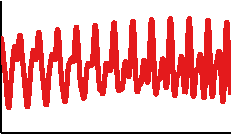
\includegraphics[width=0.2\textwidth]{figures/trans_samples/draw_21} &
      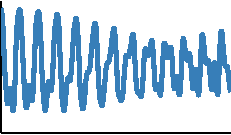
\includegraphics[width=0.2\textwidth]{figures/trans_samples/draw_22} &
      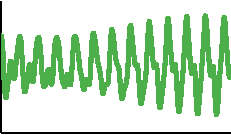
\includegraphics[width=0.2\textwidth]{figures/trans_samples/draw_23} &
      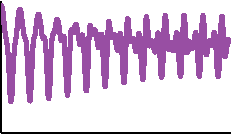
\includegraphics[width=0.2\textwidth]{figures/trans_samples/draw_24}
    \end{tabular}
  \end{block}
\end{frame}

\begin{frame}{Products of kernels - $\kLin$}
  \begin{align*}
    \underbrace{\kSE}_{\textnormal{\scriptsize approximately}} \times
    \underbrace{\kPer}_{\textnormal{\scriptsize periodic function}} \times 
    \underbrace{\kLin}_{\textnormal{\scriptsize with linearly growing amplitude}} \phantom{\times 
    \underbrace{\boldsymbol{\sigma}}_{\textnormal{\scriptsize until 1700}}}
  \end{align*}
  
  \vspace{\baselineskip}
  
  {\bf Multiplication by $\kLin$} is equivalent to multiplying the function being modeled by a linear function.
If $f(x) \,\sim\, \gp{}(0, \kernel)$, then $x\,f(x) \,\sim\, \gp{}\left(0, k \times \kLin \right)$.
This causes the standard deviation of the model to vary linearly without affecting the correlation.
  
  \vspace{\baselineskip}
  
  \begin{block}{}
    \begin{tabular}{cccc}
      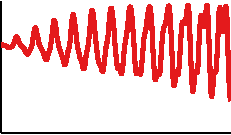
\includegraphics[width=0.2\textwidth]{figures/trans_samples/draw_31} &
      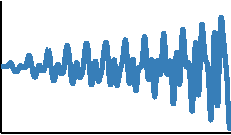
\includegraphics[width=0.2\textwidth]{figures/trans_samples/draw_32} &
      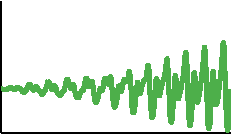
\includegraphics[width=0.2\textwidth]{figures/trans_samples/draw_33} &
      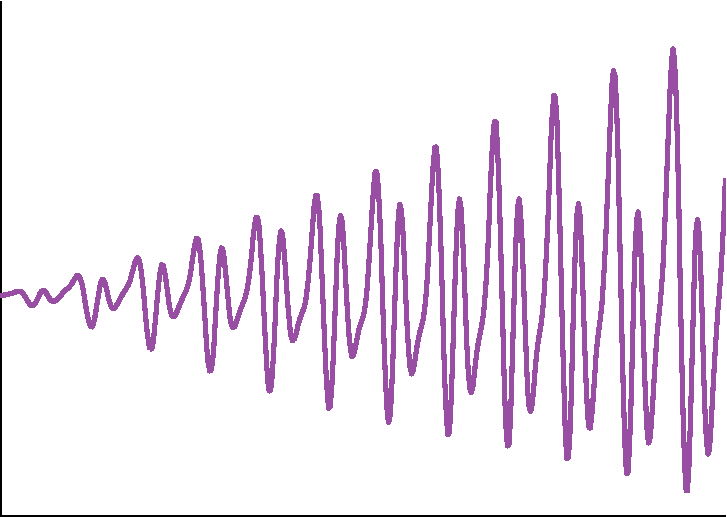
\includegraphics[width=0.2\textwidth]{figures/trans_samples/draw_34}
    \end{tabular}
  \end{block}
\end{frame}

\begin{frame}{Products of kernels - changepoints}
  \begin{align*}
    \underbrace{\kSE}_{\textnormal{\scriptsize approximately}} \times
    \underbrace{\kPer}_{\textnormal{\scriptsize periodic function}} \times 
    \underbrace{\kLin}_{\textnormal{\scriptsize with linearly growing amplitude}} \times 
    \underbrace{\boldsymbol{\sigma}}_{\textnormal{\scriptsize until 1700}}
  \end{align*}
  
  \vspace{\baselineskip}
  
  {\bf Multiplication by $\boldsymbol\sigma$} is equivalent to multiplying the function being modeled by a sigmoid.
  
  \vspace{\baselineskip}
  
  \begin{block}{}
    \begin{tabular}{cccc}
      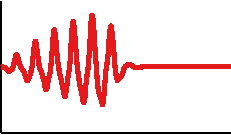
\includegraphics[width=0.2\textwidth]{figures/trans_samples/draw_41} &
      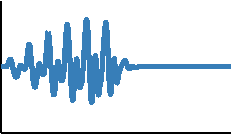
\includegraphics[width=0.2\textwidth]{figures/trans_samples/draw_42} &
      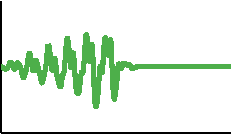
\includegraphics[width=0.2\textwidth]{figures/trans_samples/draw_43} &
      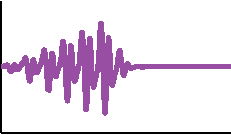
\includegraphics[width=0.2\textwidth]{figures/trans_samples/draw_44}
    \end{tabular}
  \end{block}
\end{frame}

\begin{frame}{Noun phrase and postmodifier forms}
  \begin{center}
    \footnotesize
    \begin{tabular}{l|l|l}
      Kernel & Noun phrase & Postmodifier phrase \\
      \midrule
      $\kWN$  & uncorrelated noise & n/a\\
      $\kC$   & constant & n/a \\
      $\kSE$  & smooth function & whose shape changes smoothly\\
      $\kPer$ & periodic function & modulated by a periodic function\\
      $\kLin$ & linear function & with linearly varying amplitude\\ 
      $\prod_k \kLin^{(k)}$ & polynomial & with polynomially varying amplitude\\
      $\prod_k \boldsymbol{\sigma}^{(k)}$ & n/a & which applies until / from [changepoint]
    \end{tabular}
  \end{center}
\end{frame}

\begin{frame}{Automatically generated reports}
    % Define block styles
  \tikzstyle{block} = [rectangle, draw, fill=blue!20, 
                       text width=4.4em, text centered, rounded corners, minimum height=3em]
  \tikzstyle{superblock} = [rectangle, draw, fill=blue!50, 
                       text width=4.4em, text centered, rounded corners, minimum height=3em]
  \tikzstyle{line} = [draw, -latex']
  \tikzstyle{cloud} = [draw, ellipse,fill=red!20,minimum height=2em]
  \tikzstyle{supercloud} = [draw, ellipse,fill=red!50,minimum height=2em]
    
  \begin{tikzpicture}[node distance = 2.3cm]
    \footnotesize
    % Place nodes
    \node [cloud] (data) {Data};
    \node [block, right of=data] (search) {Search};
    \node [cloud, above of=search] (language) {Language of models};
    \node [block, below of=search] (eval) {Evaluation};
    \node [cloud, right of=search] (model) {Model};
    \node [block, right of=model] (pred) {Prediction};
    \node [block, above of=pred] (trans) {Description};
    \node [block, below of=pred] (checking) {Checking};
    \node [supercloud, right of=pred] (report) {\bf Report};
    % Draw edges
    \path [line] (data) -- (search);
    \path [line] (language) -- (search);
    \path [line] (search) -- (model);
    \path [line] (search) -- (model);
    \path [line] (model.north east) -- (trans.south west);
    \path [line] (model.east) -- (pred.west);
    \path [line] (model.south east) -- (checking.north west);
    \path [line] (trans.south east) -- (report.north west);
    \path [line] (pred.east) -- (report.west);
    \path [line] (checking.north east) -- (report.south west);
    \draw[->,] (search.south east) .. controls (3.45,-1.15) .. (eval.north east);
    \draw[->,] (eval.north west) .. controls (1.15,-1.15) .. (search.south west);
  \end{tikzpicture}
\end{frame}

\begin{frame}{Example: Airline passenger volume}
\newcommand{\wmgd}{0.5\columnwidth}
\newcommand{\hmgd}{3.0cm}
\newcommand{\mdrd}{figures/01-airline}
\newcommand{\mbm}{\hspace{-0.3cm}}
\begin{tabular}{cc}
\mbm 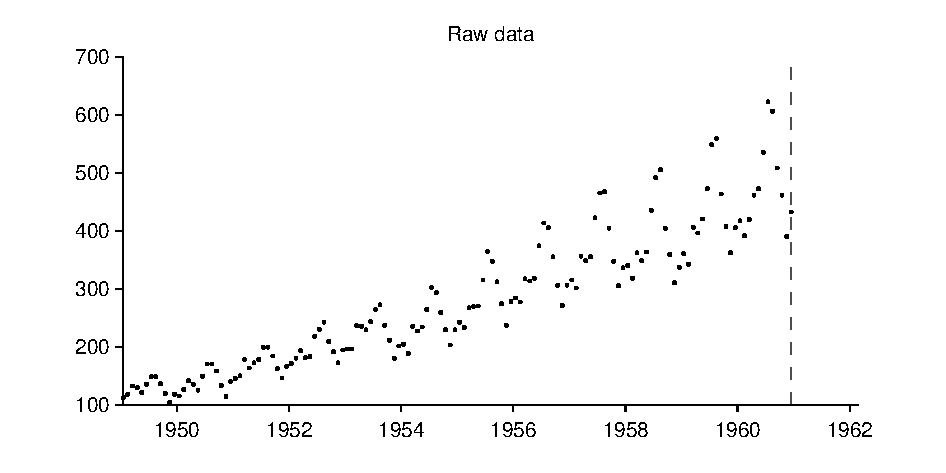
\includegraphics[width=\wmgd,height=\hmgd]{\mdrd/01-airline_raw_data} & \includegraphics[width=\wmgd,height=\hmgd]{\mdrd/01-airline_all}
\end{tabular}

{\footnotesize
Four additive components have been identified in the data
\begin{itemize}

  \item A linearly increasing function. 

  \item An approximately periodic function with a period of 1.0 years and with linearly increasing amplitude. 

  \item A smooth function. 

  \item Uncorrelated noise with linearly increasing standard deviation. 

\end{itemize}
}
\end{frame}

\begin{frame}{Example: Airline passenger volume}
\newcommand{\wmgd}{0.5\columnwidth}
\newcommand{\hmgd}{3.0cm}
\newcommand{\mdrd}{figures/01-airline}
\newcommand{\mbm}{\hspace{-0.3cm}}
{\footnotesize
This component is linearly increasing.
}

\vspace{\baselineskip}

\begin{tabular}{cc}
\mbm \includegraphics[width=\wmgd,height=\hmgd]{\mdrd/01-airline_1} & 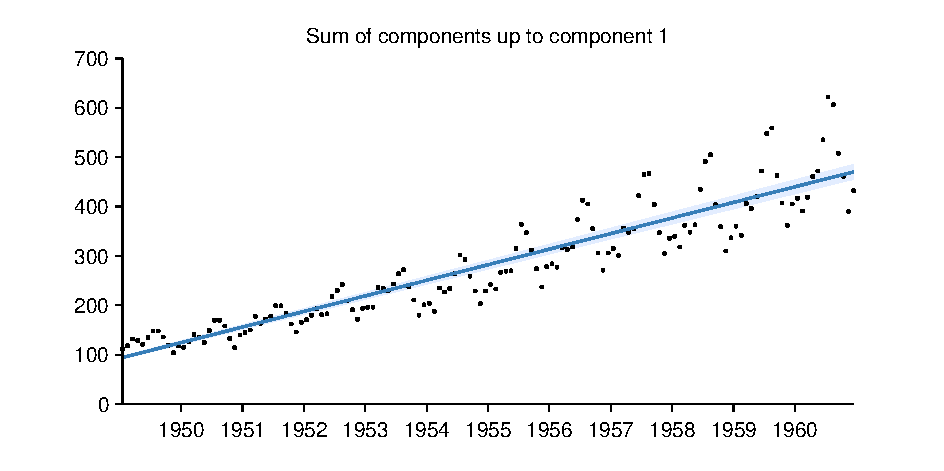
\includegraphics[width=\wmgd,height=\hmgd]{\mdrd/01-airline_1_cum}
\end{tabular}
\end{frame}

\begin{frame}{Example: Airline passenger volume}
\newcommand{\wmgd}{0.5\columnwidth}
\newcommand{\hmgd}{3.0cm}
\newcommand{\mdrd}{figures/01-airline}
\newcommand{\mbm}{\hspace{-0.3cm}}
{\footnotesize
This component is approximately periodic with a period of 1.0 years and varying amplitude.
Across periods the shape of this function varies very smoothly.
The amplitude of the function increases linearly.
The shape of this function within each period has a typical lengthscale of 6.0 weeks.
}

\vspace{\baselineskip}

\begin{tabular}{cc}
\mbm \includegraphics[width=\wmgd,height=\hmgd]{\mdrd/01-airline_2} & 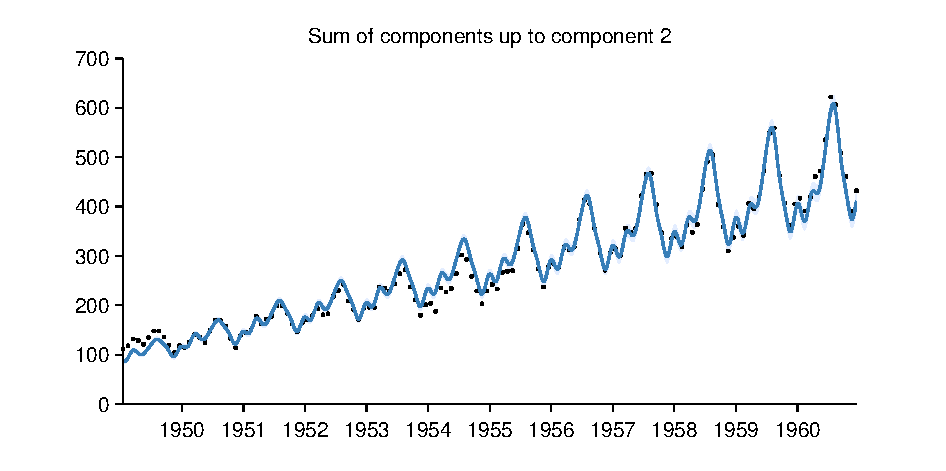
\includegraphics[width=\wmgd,height=\hmgd]{\mdrd/01-airline_2_cum}
\end{tabular}
\end{frame}

\begin{frame}{Example: Airline passenger volume}
\newcommand{\wmgd}{0.5\columnwidth}
\newcommand{\hmgd}{3.0cm}
\newcommand{\mdrd}{figures/01-airline}
\newcommand{\mbm}{\hspace{-0.3cm}}
{\footnotesize
This component is a smooth function with a typical lengthscale of 8.1 months.
}

\vspace{\baselineskip}

\begin{tabular}{cc}
\mbm \includegraphics[width=\wmgd,height=\hmgd]{\mdrd/01-airline_3} & 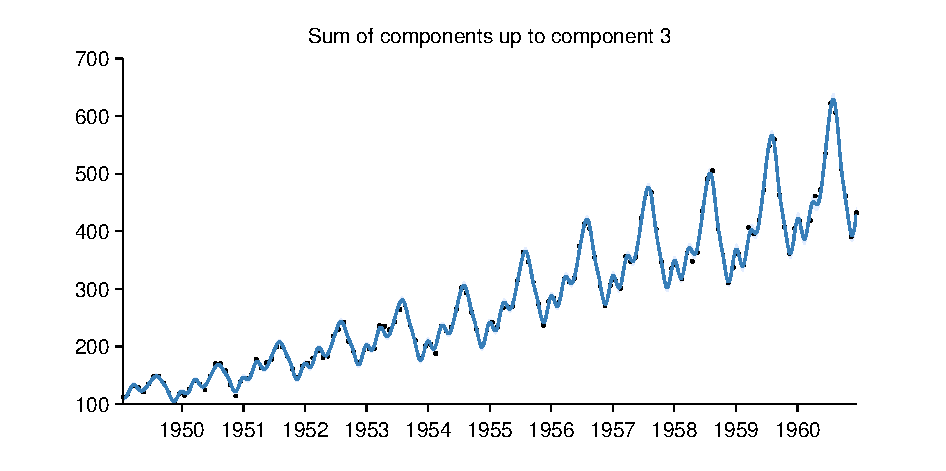
\includegraphics[width=\wmgd,height=\hmgd]{\mdrd/01-airline_3_cum}
\end{tabular}
\end{frame}

\begin{frame}{Example: Airline passenger volume}
\newcommand{\wmgd}{0.5\columnwidth}
\newcommand{\hmgd}{3.0cm}
\newcommand{\mdrd}{figures/01-airline}
\newcommand{\mbm}{\hspace{-0.3cm}}
{\footnotesize
This component models uncorrelated noise.
The standard deviation of the noise increases linearly.
}

\vspace{\baselineskip}

\begin{tabular}{cc}
\mbm 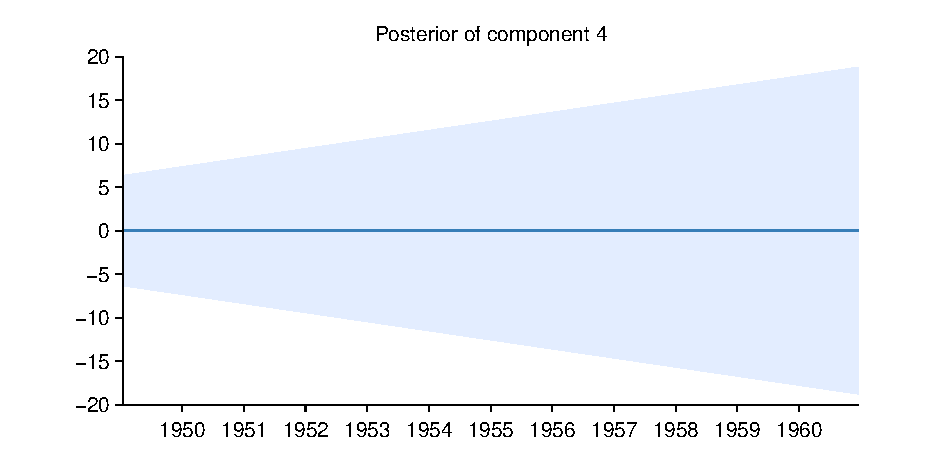
\includegraphics[width=\wmgd,height=\hmgd]{\mdrd/01-airline_4} & 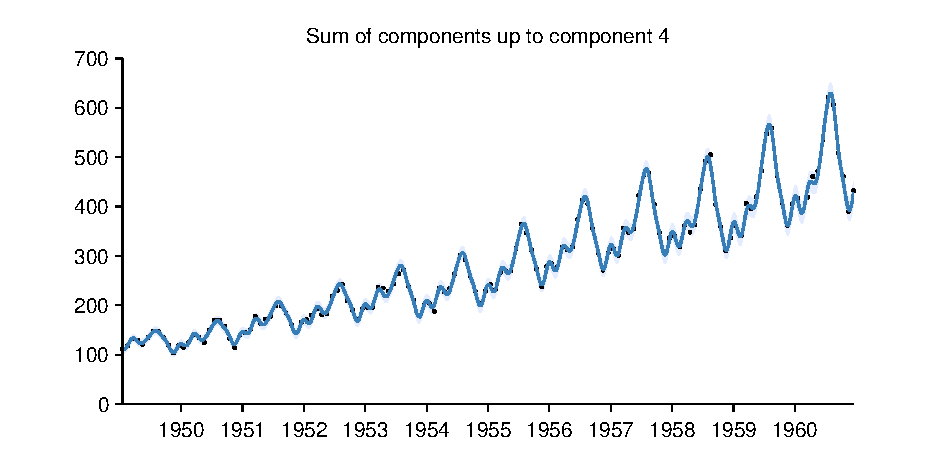
\includegraphics[width=\wmgd,height=\hmgd]{\mdrd/01-airline_4_cum}
\end{tabular}
\end{frame}

\begin{frame}{Example: Solar irradiance}
\newcommand{\wmgd}{0.5\columnwidth}
\newcommand{\hmgd}{3.0cm}
\newcommand{\mdrd}{figures/02-solar}
\newcommand{\mbm}{\hspace{-0.3cm}}
{\footnotesize
This component is constant.
}

\vspace{\baselineskip}

\begin{tabular}{cc}
\mbm 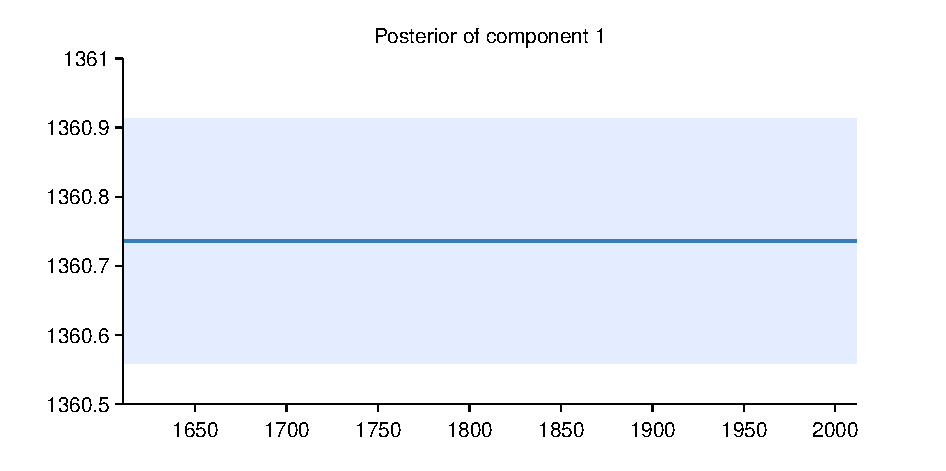
\includegraphics[width=\wmgd,height=\hmgd]{\mdrd/02-solar_1} & \includegraphics[width=\wmgd,height=\hmgd]{\mdrd/02-solar_1_cum}
\end{tabular}
\end{frame}

\begin{frame}{Example: Solar irradiance}
\newcommand{\wmgd}{0.5\columnwidth}
\newcommand{\hmgd}{3.0cm}
\newcommand{\mdrd}{figures/02-solar}
\newcommand{\mbm}{\hspace{-0.3cm}}
{\footnotesize
This component is constant.
This component applies from 1643 until 1716.
}

\vspace{\baselineskip}

\begin{tabular}{cc}
\mbm \includegraphics[width=\wmgd,height=\hmgd]{\mdrd/02-solar_2} & \includegraphics[width=\wmgd,height=\hmgd]{\mdrd/02-solar_2_cum}
\end{tabular}
\end{frame}

\begin{frame}{Example: Solar irradiance}
\newcommand{\wmgd}{0.5\columnwidth}
\newcommand{\hmgd}{3.0cm}
\newcommand{\mdrd}{figures/02-solar}
\newcommand{\mbm}{\hspace{-0.3cm}}
{\footnotesize
This component is a smooth function with a typical lengthscale of 23.1 years.
This component applies until 1643 and from 1716 onwards.
}

\vspace{\baselineskip}

\begin{tabular}{cc}
\mbm \includegraphics[width=\wmgd,height=\hmgd]{\mdrd/02-solar_3} & \includegraphics[width=\wmgd,height=\hmgd]{\mdrd/02-solar_3_cum}
\end{tabular}
\end{frame}

\begin{frame}{Example: Solar irradiance}
\newcommand{\wmgd}{0.5\columnwidth}
\newcommand{\hmgd}{3.0cm}
\newcommand{\mdrd}{figures/02-solar}
\newcommand{\mbm}{\hspace{-0.3cm}}
{\footnotesize
This component is approximately periodic with a period of 10.8 years.
Across periods the shape of this function varies smoothly with a typical lengthscale of 36.9 years.
The shape of this function within each period is very smooth and resembles a sinusoid.
This component applies until 1643 and from 1716 onwards.
}

\vspace{\baselineskip}

\begin{tabular}{cc}
\mbm \includegraphics[width=\wmgd,height=\hmgd]{\mdrd/02-solar_4} & \includegraphics[width=\wmgd,height=\hmgd]{\mdrd/02-solar_4_cum}
\end{tabular}
\end{frame}

\begin{frame}{Model checking / criticism}
    % Define block styles
  \tikzstyle{block} = [rectangle, draw, fill=blue!20, 
                       text width=4.4em, text centered, rounded corners, minimum height=3em]
  \tikzstyle{superblock} = [rectangle, draw, fill=blue!50, 
                       text width=4.4em, text centered, rounded corners, minimum height=3em]
  \tikzstyle{line} = [draw, -latex']
  \tikzstyle{cloud} = [draw, ellipse,fill=red!20,minimum height=2em]
  \tikzstyle{supercloud} = [draw, ellipse,fill=red!50,minimum height=2em]
    
  \begin{tikzpicture}[node distance = 2.3cm]
    \footnotesize
    % Place nodes
    \node [cloud] (data) {Data};
    \node [block, right of=data] (search) {Search};
    \node [cloud, above of=search] (language) {Language of models};
    \node [block, below of=search] (eval) {Evaluation};
    \node [cloud, right of=search] (model) {Model};
    \node [block, right of=model] (pred) {Prediction};
    \node [block, above of=pred] (trans) {Description};
    \node [superblock, below of=pred] (checking) {Checking};
    \node [cloud, right of=pred] (report) {Report};
    % Draw edges
    \path [line] (data) -- (search);
    \path [line] (language) -- (search);
    \path [line] (search) -- (model);
    \path [line] (search) -- (model);
    \path [line] (model.north east) -- (trans.south west);
    \path [line] (model.east) -- (pred.west);
    \path [line] (model.south east) -- (checking.north west);
    \path [line] (trans.south east) -- (report.north west);
    \path [line] (pred.east) -- (report.west);
    \path [line] (checking.north east) -- (report.south west);
    \draw[->,] (search.south east) .. controls (3.45,-1.15) .. (eval.north east);
    \draw[->,] (eval.north west) .. controls (1.15,-1.15) .. (search.south west);
  \end{tikzpicture}
\end{frame}

\begin{frame}{Is this model `correct'?}
\newcommand{\wmgd}{0.5\columnwidth}
\newcommand{\hmgd}{3.0cm}
\newcommand{\mdrd}{figures/11-unemployment}
\newcommand{\mbm}{\hspace{-0.3cm}}
\begin{tabular}{cc}
\mbm \includegraphics[width=\wmgd,height=\hmgd]{\mdrd/11-unemployment_raw_data} & \includegraphics[width=\wmgd,height=\hmgd]{\mdrd/11-unemployment_all}
\end{tabular}

{\footnotesize
\begin{itemize}

  \item A very smooth monotonically increasing function. 

  \item An approximately periodic function with a period of 1.0 years. 

  \item A smooth function. 

  \item A smooth function. 

  \item Uncorrelated noise. 

\end{itemize}
}
\end{frame}

\begin{frame}{Model criticism}
  \begin{itemize}
    \item Model criticism attempts to answer the question `Is this model wrong?'
    \begin{itemize}
      \item Formalised as, `could the data have been generated by this model?'
    \end{itemize}
    \vspace{\baselineskip}
    \item Typically answered by choosing a statistic by which to measure whether data is extreme
    \begin{itemize}
      \item Can then compute $p$-values to quantify surprise
      \item $p(\textrm{Data}) = \mathbb{P}(T(\textrm{Hypothetical data}) > T(\textrm{Data}) \,|\, \textrm{Model})$
    \end{itemize}
    \vspace{\baselineskip}
    \item How would an automatic system choose this statistic?
  \end{itemize}
\end{frame}

\begin{frame}{Potential solution: Try many statistics}

\begin{itemize}
  \item $p$-values of several statistics for each model component
\end{itemize}

\vspace{\baselineskip}

\begin{center}
\begin{tabular}{|r|rr|rr|rr|}
\hline
 & \multicolumn{2}{c|}{ACF} & \multicolumn{2}{c|}{Periodogram} & \multicolumn{2}{c|}{QQ} \\
\bf{\#} & {min} & {min loc} & {max} & {max loc} & {max} & {min}\\
\hline

1 & \textcolor{gray}{0.502} & \textcolor{gray}{0.582} & \textcolor{gray}{0.341} & \textcolor{gray}{0.413} & \textcolor{gray}{0.341} & \textcolor{gray}{0.679}\\

2 & \textcolor{gray}{0.802} & \textcolor{gray}{0.199} & \textcolor{gray}{0.558} & \textcolor{gray}{0.630} & 0.049 & \textcolor{gray}{0.785}\\

3 & \textcolor{gray}{0.251} & \textcolor{gray}{0.475} & \textcolor{gray}{0.799} & \textcolor{gray}{0.447} & \textcolor{gray}{0.534} & \textcolor{gray}{0.769}\\

4 & \textcolor{gray}{0.527} & \textcolor{gray}{0.503} & \textcolor{gray}{0.504} & \textcolor{gray}{0.481} & \textcolor{gray}{0.430} & \textcolor{gray}{0.616}\\

5 & \textcolor{gray}{0.493} & \textcolor{gray}{0.477} & \textcolor{gray}{0.503} & \textcolor{gray}{0.487} & \textcolor{gray}{0.518} & \textcolor{gray}{0.381}\\

\hline
\end{tabular}
\end{center}

\end{frame}

\begin{frame}{Example: Identifying outliers}
  \newcommand{\wmgd}{0.5\columnwidth}
  \newcommand{\hmgd}{3.0cm}
  \newcommand{\mdrd}{figures/11-unemployment} 
  \newcommand{\mbm}{\hspace{-0.3cm}}
The following discrepancies between the prior and posterior distributions for this component have been detected.
\begin{itemize}
    \item The qq plot has an unexpectedly large positive deviation from equality ($x = y$). This discrepancy has an estimated $p$-value of 0.049.
\end{itemize}

\vspace{\baselineskip}

\begin{tabular}{cc}
\mbm \includegraphics[width=\wmgd,height=\hmgd]{\mdrd/11-unemployment_2} & 
\mbm \includegraphics[width=\wmgd,height=\hmgd]{\mdrd/11-unemployment_qq_bands_2}
\end{tabular}
\end{frame}

\begin{frame}{Alternatives to choosing one statistic}
  \begin{itemize}
    \item Compute many statistics with appropriate multiple comparisons adjustments
    \vspace{\baselineskip}
    \item Something nonparametric?
    \vspace{\baselineskip}
    \item Some sort of grammar based search over statistics?
  \end{itemize}
\end{frame}

\begin{frame}{A nonparametric approach}
  \begin{itemize}
    \item Instead of defining a statistic parametrically to measure a discrepancy, we pick the statistic that most shows any discrepancy
    \vspace{\baselineskip}
    \item Based on the maximum mean discrepancy between two distributions
    \begin{itemize}
      \item $\textrm{MMD}(\mathcal{F},p,q) = \sup_{f \in \mathcal{F}}(\mathbb{E}_{x\sim p}[f(x)] - \mathbb{E}_{y\sim q}[f(y)])$ where $\mathcal{F}$ is a set of functions
    \end{itemize}
    \vspace{\baselineskip}
    \item The function attaining the supremum can be computed analytically when $\mathcal{F}$ is an RKHS
    \begin{itemize}
      \item $f(x) = \mathbb{E}_{x'\sim p}[k(x,x')] - \mathbb{E}_{x'\sim q}[k(x,x')]$
    \end{itemize}
  \end{itemize}
\end{frame}

\begin{frame}{Example}
  \begin{center}
  \begin{tabular}{cc}
    \includegraphics[width=0.435\textwidth]{figures/newcomb_hist} &
    \includegraphics[width=0.48\textwidth]{figures/newcomb_witness_1}
  \end{tabular}
  \end{center}
\end{frame}

\begin{frame}{What next for the automatic statistician?}
 \begin{itemize}
   \item Plenty of ways to extend this line of work \eg
   \begin{itemize}
     \item Reducing the computational cost of model search
     \item Increasing the expressivity of the modelling language (\eg monotonicity, positive functions)
     \item Extending descriptions to multi-dimensional functions
     \item Different likelihoods
     \item Different types of data (\eg exchangeable arrays)
     \item Missing data
     \item \dots
   \end{itemize}
   \vspace{\baselineskip}
   \item How can we tie the automatic statistician project together?
 \end{itemize}
\end{frame}

\begin{frame}{An API for the automatic statistician}
  \begin{itemize}
    \item Many automatic / standardised tools for machine learning
    \begin{itemize}
      \item Goole prediction API, scikit-learn, auto-WEKA, \dots
    \end{itemize}
    \vspace{\baselineskip}
    \item Focused on prediction, essentially implementing the following functions
    \begin{itemize}
      \item train
      \item predict
    \end{itemize}
    \vspace{\baselineskip}
    \item Let's implement some more functions
    \begin{itemize}
      \item describe
      \item criticise
    \end{itemize}
  \end{itemize}
\end{frame}

\begin{frame}{Thanks}
  \begin{center}
  \Huge
  Thanks
  \end{center}
\end{frame}

\begin{frame}{Appendix}
\end{frame}

\begin{frame}{Gaussian processes}
  \begin{itemize}
    \item A Gaussian process is collection of random variables, any finite number of which have a joint Gaussian distribution
    \pause
    \vspace{\baselineskip}
    \item We can write this collection of random variables as $\{f(x) : x \in \mathcal{X}\}$ \ie a function $f$ evaluated at inputs $x$
    \pause
    \vspace{\baselineskip}
    \item A \gp{} is completely specified by
    \begin{itemize}
      \item Mean function, $\mu(x)=\mathbb{E}(f(x))$
      \item Covariance / kernel function, $\kernel(x,x') = \Cov(f(x),f(x'))$
      \item Denoted $f \,\sim\, \gp{}(\mu,\kernel)$
    \end{itemize}
    \vspace{\baselineskip}
    \pause
    \item Can be thought of as a probability distribution on functions
  \end{itemize}
\end{frame}

\begin{frame}{A language of Gaussian process kernels}
  \begin{itemize}
    \item It is common practice to use a zero mean function since the mean can be marginalised out
  \begin{itemize}
    \item Suppose, ${f(x) \,|\, a \,\sim\, \gp{}(a \times \mu(x), \kernel(x,x'))}$ where $a \,\sim\, \mathcal{N}(0,1)$
    \item Then equivalently, $f(x) \,\sim\, \gp{}(0, \mu(x)\mu(x') + \kernel(x,x'))$
  \end{itemize}
  \vspace{\baselineskip}
  \item We therefore define a language of \gp{} regression models by
specifying a {\bf language of kernels}
  \end{itemize}
\end{frame}

\end{document}

\begin{frame}{Title}
  \begin{itemize}
    \item Content
    \vspace{\baselineskip}
    \item Content
    \vspace{\baselineskip}
    \item Content
    \begin{itemize}
       \item Content
       \item Content
     \end{itemize}
  \end{itemize}
\end{frame}
